\chapter{Evaluierung}

\section{Benutzerevaluierung}
\paragraph{}
Damit es festgestellt werden könnte, ob die Anreicherung von Suchergebnissen mit aus den Snippets extrahierten Entitäten für den Benutzer auch tatsächlich hilfreich sein könnte, wurde eine Benutzerevaluierung durchgeführt. Die Evaluierung sollte folgende Fragen beantworten:

\begin{itemize}
\item Welcher Einsatz liefert dem Benutzer die zu der Anfrage am besten passende Entitäten? 
\item Wird die Geschwindigkeit der Suche durch zusätzlicher Schritt der Extraktion von Entitäten stark beeinträchtigt? Ist die Beeinträchtigung der Geschwindigkeit groß Genug, um den Benutzer bei der Suche zu stören?
\item Gibt es Korrelationen zwischen ,,standarten`` Metriken wie F-Measure und Precision/Recall und der Zufriedenheit der Benutzer, oder kann man aus der rein numerischen Metriken keine Aussage treffen, ob der Engine in der Lage ist, eine genügende Benutzerunterstützung zu leisten?
\end{itemize}

Um diese Fragen beantworten zu können, wurde eine Webseite aufgebaut, die dem Benutzer die Möglichkeit gibt, alle Engines und alle Modellen, die im Rahmen dieser Arbeit verwendet wurden, zu bewerten. Insgesamt kann der Evaluirungsvorgang in drei Schritten geteilt werden:

\begin{enumerate}
\item In dem Einleitungsschritt wird dem Benutzer erklärt, wie genau die Evaluierung abläuft, und was wir von ihm brauchen.
\item Danach muss der Benutzer alle vorhandene Kombinationen von Modellen und Engines bewerten. Dazu soll eine Frage aus der vorgegebenen Liste ausgewählt und gestellt werden, die zuerst an Bing gesendet wird, und dann an unseres Stanbol-Backend.
\item Um die Situation, wo der Benutzer sich ,,betrogen`` fühlen könnte, möglichst auszuschließen, wird dem Probanden die Möglichkeit gegeben, jede beliebige Frage zu stellen, und dann einen persönlichen schriftlichen Feedback abzugeben.
\end{enumerate}

\begin{figure}
\centering
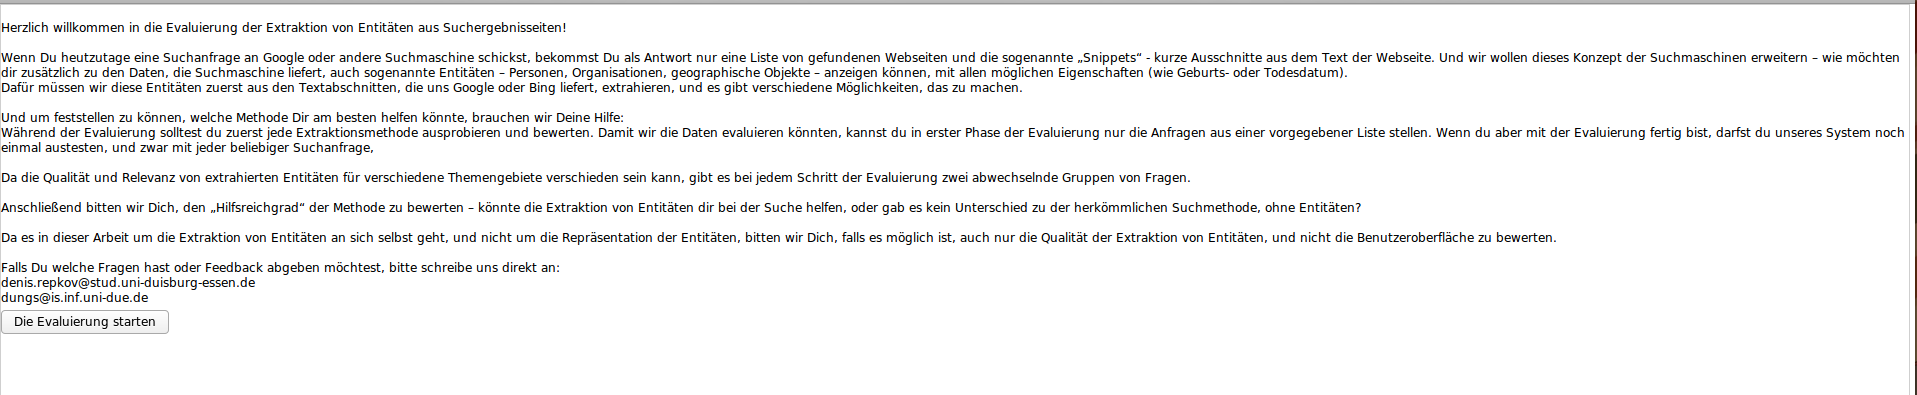
\includegraphics[width=1.0\textwidth]{Bilder/evalstep1.png}
\caption{''Einleitung in die Evaluierung''}
\label{fig:evalstep01}
\end{figure}

\begin{figure}
\centering
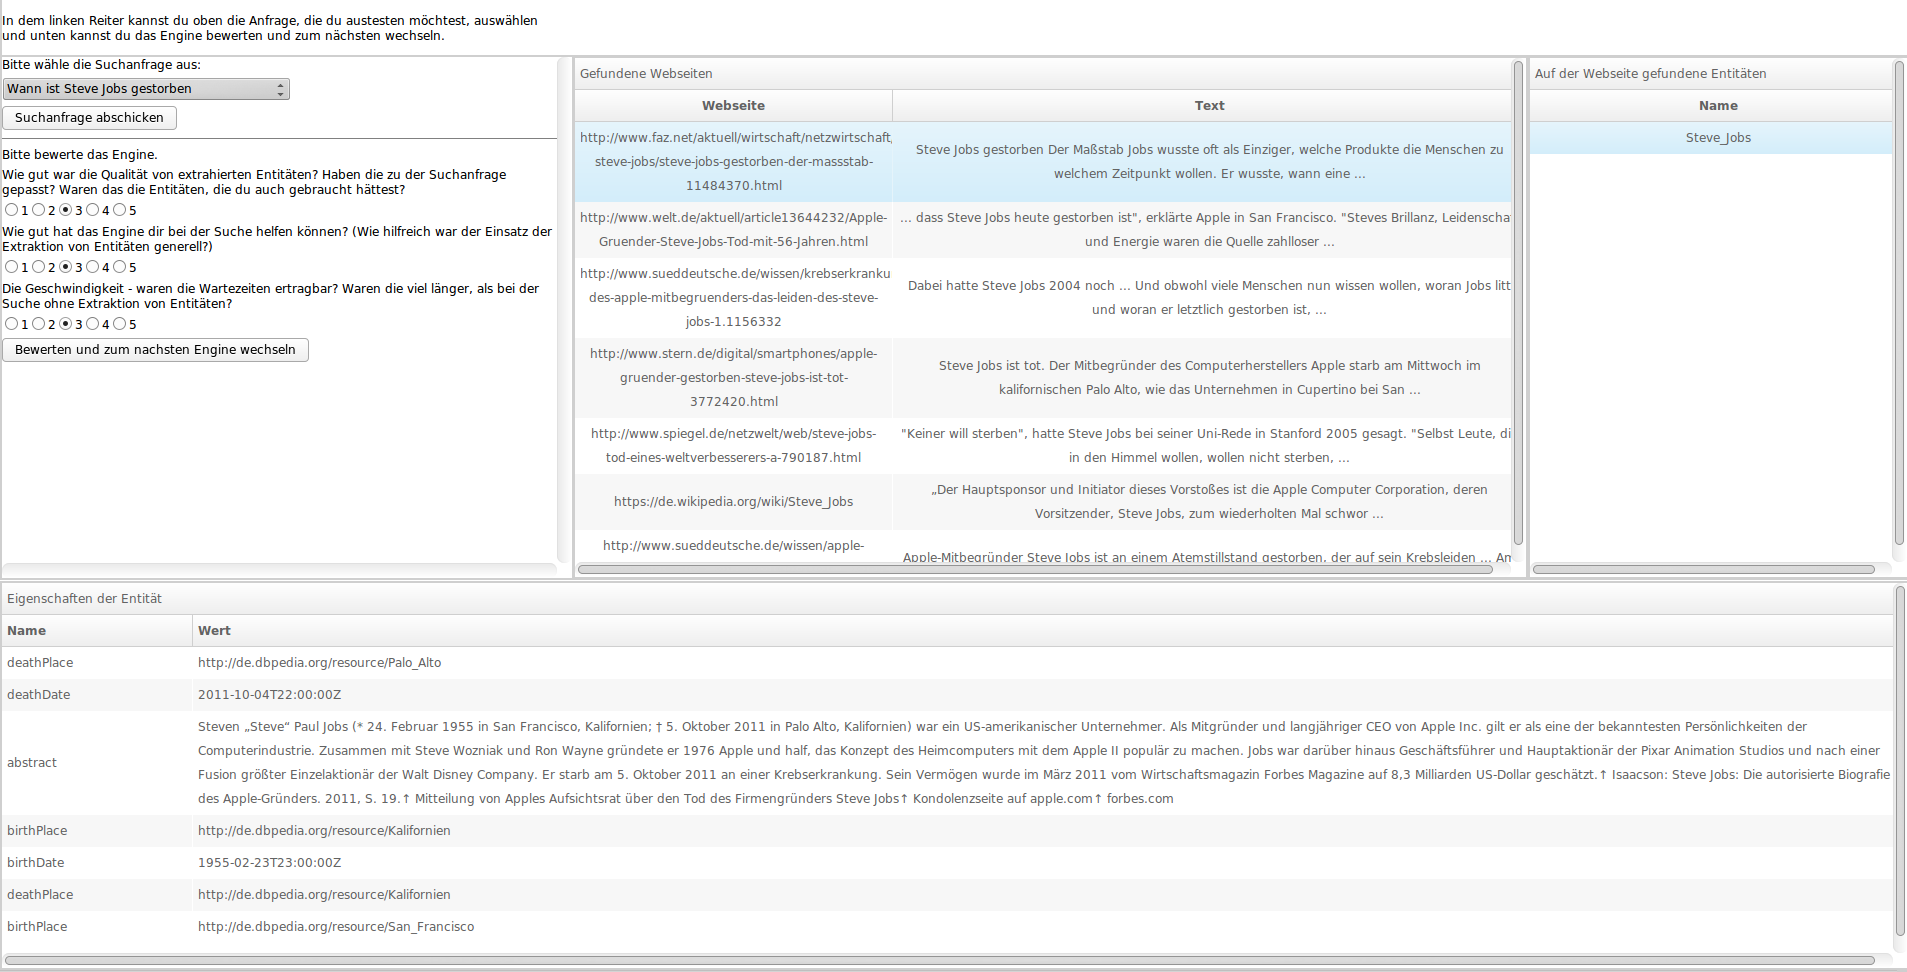
\includegraphics[width=1.0\textwidth]{Bilder/evalstep2.png}
\caption{''Bewertung eines Engines''}
\label{fig:evalstep01}
\end{figure}

\begin{figure}
\centering
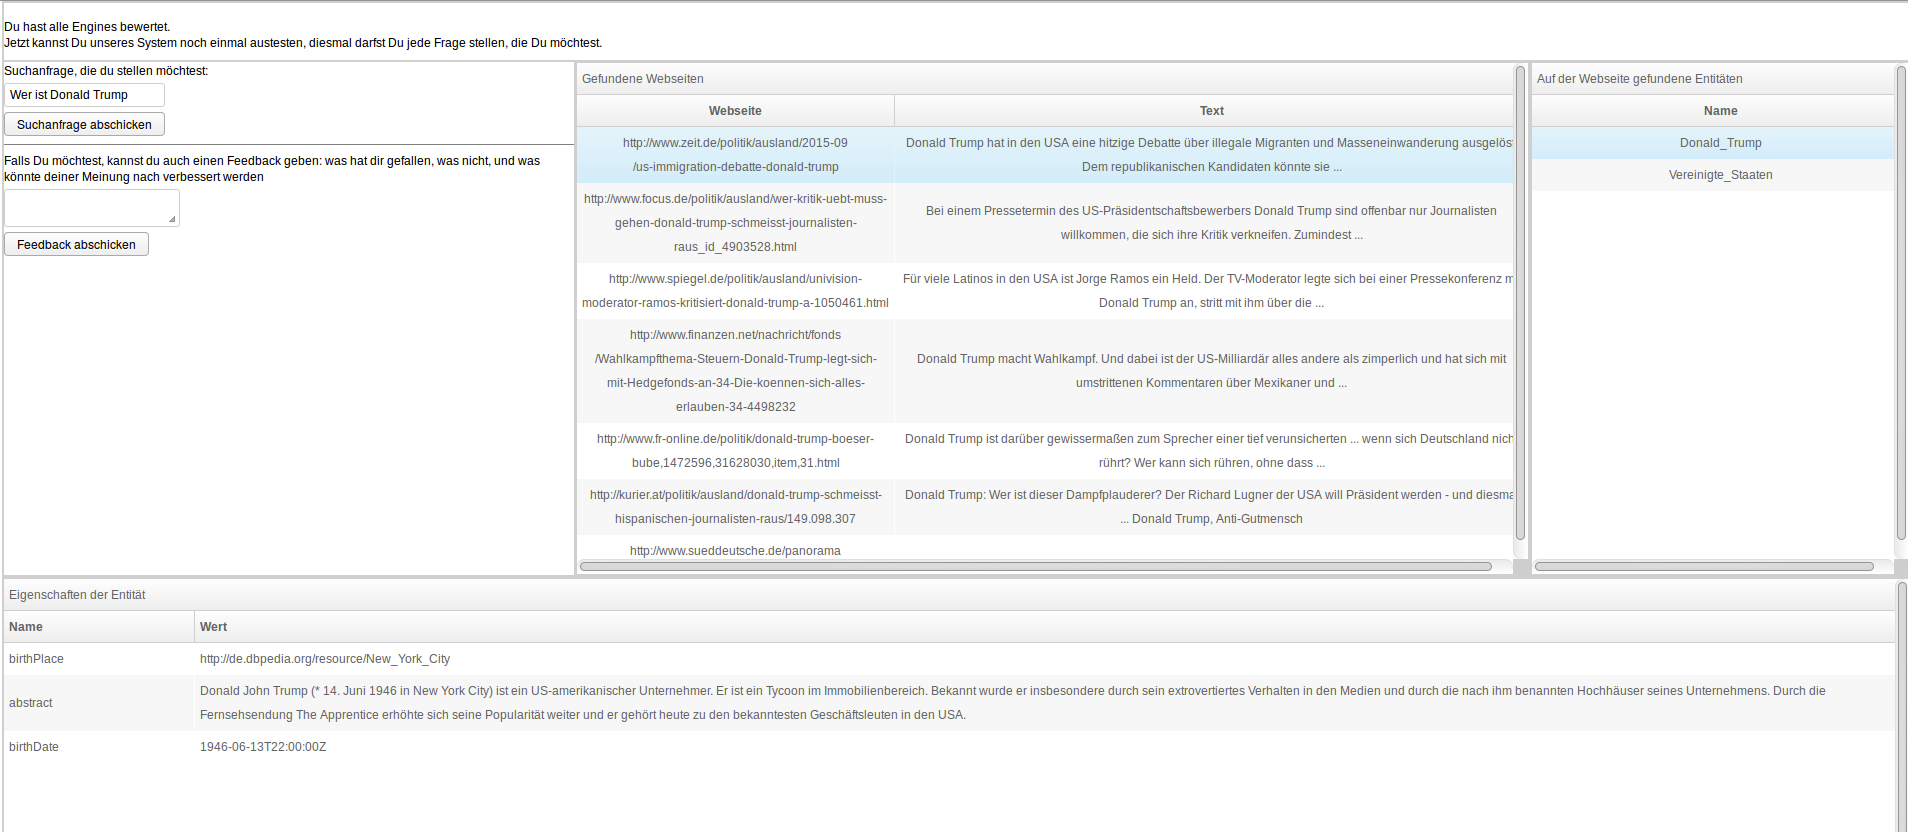
\includegraphics[width=1.0\textwidth]{Bilder/evalstep3.png}
\caption{''Der letzte Schritt der Evaluierung''}
\label{fig:evalstep01}
\end{figure}

Für jedes Engine sollen insgesamt drei Charakteristiken bewertet werden:
\begin{enumerate}
\item Qualität von extrahierten Entitäten - der Benutzer soll beschreiben, wie gut seiner Meinung nach die Entitäten zu den extrahierten Snippets gepasst haben, ob diese ,,korrekt`` von dem Gesichtspunkt des Probanden waren, ob es für die gefundene Entitäten die Daten vorhanden sind, die der Benutzer auch wirklich braucht, und ob es die Informationen gibt, die für die Suche eigentlich kaum zu Nutzen sind.
\item Geschwindigkeit der Anreicherung - Der Proband soll angeben, ob die die Extraktion von Entitäten mit der Suche zusammen schnell genug waren, besonders im Vergleich zu den Suchmaschinen wie Google oder Bing.
\item ,,Hilfreichsgrad`` von dem Ansatz - Damit soll der Benutzer uns mitteilen, ob solch eine Anreicherung von herkömmlichen Suchergebnissen mit den Entitäten und dazugehörigen Informationen wie Geburtstag/Geburtsort/u.s.w. für die Präzision der Suchanfrage hilfreich wäre, und ob der Proband den Einsatz dieser Suchmethode sinnvoll fände.  
\end{enumerate}

\section{Automatisierte Evaluierung von Qualität der Extraktion}
\paragraph{}
Es stellt sich allerdings die Frage, ob die aus der Benutzerstudie gewonnene Ergebnisse mit den in natürsprachlicher Mensch-Computer-Interaktion übliche Evaluierungsmethoden wie 
\begin{itemize}
\item Präzision
\item Recall
\item F-Measure
\end{itemize}
vereinbart werden könnten? Was ist für den Benutzer wichtige - dass das Engine so wenig False-Positiv-Treffer wie möglich liefert, oder ob die FP für den Benutzer ehe keine bedeutende Rolle spielen? Kann man anhand statistischen Messdaten sagen können, ob das Engine auch aus Sicht des Benutzers positiv oder negativ bewertet wird? Um diese Fragen beantworten zu können, müssen noch statistische Messungen durchgeführt werden und ihre Ergebnisse mit den aus der Benutzerevaluierung gewonnenen Daten vergleichen.

\section{Diskussion}
\paragraph{}
Während der Studie wurden insgesamt 44 Bewertungen gesammelt, deren Ergebnisse in der Tabelle \ref{table:RESULTS} zu sehen sind. Es wurden außerdem einige Feedbacks gesammelt, die für die Analyse der Arbeit und als Quelle für Verbesserungsvorschläge verwendet werden können. Die Liste von Feedbacks findet man in der Auflistung \ref{lst:feedbacks}. Aber welche Schlussfolgerungen lassen sich daraus ziehen? Auf den ersten Blick fallen folgende Besonderheiten auf:
\begin{itemize}
\item Die Benutzer fanden den Einsatz hilfreich, wünschen sich aber die Verbesserung von dem Benutzerinterface des Systems.
\item Es werden eventuell zu viel Informationen angezeigt, so dass der Benutzer sich verwirrt fühlen könnte.
\item Die Probanden fanden die Geschwindigkeit der Suche gut, auch wenn es definitiv länger als eine Suche mit herkömmlichen Suchmaschinen dauert. 
\item Die Benutzer bewerteten die Qualität von extrahierten Entitäten meistens als ,,nicht ausreichend``.
\end{itemize}

Es stellt sich die Frage, was bedeuten diese Ergebnisse, und was man daraus lernen kann, und welche Aspekte des entwickelten Systems sich verbessern lassen.

Die interessanteste Frage wäre, warum die Benutzer einerseits die Qualität von den extrahierten Entitäten als ,,schlecht`` bewertet haben, aber anderseits den Einsatz von Entitäten als ,,hilfreich`` bezeichneten, und welchen Zusammenhang zwischen diesen beiden Kriterien besteht? 

Um diese Frage beantworten zu können muss es zuerst über die Definition von ,,Qualität`` von Entitäten im Rahmen der Evaluierung nachgedacht werden. In der Einleitung zur Evaluierung wurde Qualität als ,,wie gut \textbf{aus Sicht des Probanden} die Entität zu den gefundenen Snippets passt`` definiert. Das Problem hier ist, dass verschiedene Benutzer verschiedene persönliche Definitionen von den Begriffen ,,passend`` und ,,unpassend`` haben - z.B. wird aus einem Snippet zur Anfrage ,,Geburtstag von Angela Merkel`` auch die Entitäten ,,Deutschland`` und ,,CDU`` extrahiert, neben der Entität ,,Angela Merkel``, die für die Beantwortung der Anfrage eigentlich ausreichend wäre. Einige Probanden können die zwei zusätzliche Entitäten als ,,passend`` einstufen, da die zum Themengebiet des Snippet-Textes passen, aber andere Benutzer würden dieselbe Daten als ,,unpassend`` bezeichnen, da die keine Antwort auf die gestellte Frage geben. Außerdem sind die Methoden zur Extraktion von Entitäten nicht perfekt, und können im Text vorhandene Entitäten nicht immer richtig erkennen. Die Rolle vom Trainingskorpus soll auch im Kauf genommen werden - automatisch generierte Korpora sollen generell nur dann verwendet werden, wenn keine weitere Korpora verfügbar sind (aus finanziellen Gründen z.B.).

Ein weiteres Problem kann auf die Suchmaschine zurückgeführt werden, die als Quelle für Snippets verwendet wird - auch wenn in den Suchparametern der Suchmaschine explizit mitgeteilt wird, dass es nach deutschsprachigen Seiten gesucht werden muss, werden oft auch englischsprachige Webseiten gefunden, und da das im Rahmen dieser Arbeit entwickeltes System nur für deutsche Sprache funktionieren soll, werden nicht alle von der Suchmaschine erhaltene Ergebnisse mit den Entitäten angereichert.

Die Andere Quelle für die Bewertung von extrahierten Entitäten als ,,unpassend`` können die in den dem Benutzer gezeigten Ontologien vorhandene Informationen sein. Als Erstes haben einige Benutzer bemerkt, dass es auch die Eigenschaften angezeigt werden, die mit der eigentlichen Suchanfrage nichts gemeinsames haben - z.B. auch wenn man die Informationen übers Geburtsort einer Person sucht, werden für die extrahierte Entität alle in der Wissendatenbank vorhandene Informationen angezeigt - Geburtstag, Name, Beschreibung u.s.w. Das kann zur Verwirrung führen, und somit wird die Entität als ,,schlecht`` eingestuft. Zweitens, sind die in DBpedia vorhandene Daten nicht immer vollständig - bei den Daten fürs indische Ozean fehlen z.B. die Angaben zur Fläche, da die direkt in der Kurzbeschreibung der Entität zu finden sind. Das kann eventuell dazu führen, dass der Benutzer sich in die Beschreibung der extrahierten Entität einlesen muss, und somit mehr Aufwand für die Suche anzuwenden braucht als es vorgesehen wurde. 

Ein weiterer Grund, warum die Entitäten als ,,nicht ausreichend gut`` bewertet wurden, könnte das User-Interface des Bewertungssystems sein - da das Ziel dieser Arbeit die Entwicklung des Backeds und der API für die Extraktion von Entitäten aus Suchergebnisseiten war, und die UI nur für die Durchführung der Evaluierung entwickelt wurde, wurde eine grundlegende Untersuchung, wie die Daten dem Benutzer am Besten angezeigt und dargestellt werden könnten, absichtlich nicht durchgeführt, damit der Zeitplan eingehalten werden könnte. Und obwohl es gebeten wurde, nicht die UI, sondern nur die Extraktion von Entitäten an sich selbst zu bewerten, beeinflusst die UI die Entscheidung des Benutzers trotzdem. 

\subsection{Verbesserungsvorschläge und Anregungen für die Zukunft}
Nachdem die Ergebnisse der Studie analysiert wurden, kommt die Frage, ob das System sich verbessern lässt und wie genau könnten die beschriebene Mängel beseitigt oder umgegangen werden.

Zuerst sollte das Problem von ,,unpassenden`` oder im Text vorhandenen aber nicht gefundenen Entitäten angegangen werden. Auf den ersten Blick würde sich dieses Problem durch Verwendung von größeren und besser strukturierten Korpora fürs Training des Modells lösen lassen, was allerdings das Hauptproblem - die Individualität von den Begriffen ,,passend`` und ,,unpassend`` nicht beseitigen kann.

Um das Problem von individuellen Vorstellungen des Benutzers bezüglich ,,Qualität`` von extrahierten Entitäten umzugehen, wäre folgende Lösung zumutbar: wie erwähnt, werden extrahierte Entitäten bevor die an den Snippet angehängt und zu dem Benutzer geschickt werden durch ein Filter anhand ihres Gewichtes ,,abgesiebt`` - alle Entitäten, deren Gewicht kleiner als $n$ ist, werden dem Benutzer nicht angezeigt. Da in dem entwickelten System dieses Schwellwert von dem Entwickler statisch festgesetzt wird, kommt es oft vor, dass entweder ,,unwichtige`` Entitäten angezeigt werden oder dass ,,wichtige`` Entitäten weggeworfen werden. Dieses Wert muss allerdings nicht unbedingt fest sein, und kann mithilfe einer Rückkopplung dynamisch angepasst werden, auf zwei Arten und Weisen:
\begin{enumerate}
\item Jeder Benutzer bekommt ein personalisiertes Schwellwert. Der Vorteil dieser Methode ist, dass solche Suche wirklich ,,personalisiert`` sein würde. Der Nachteil wäre die Notwendigkeit, den Benutzer zu identifizieren, was eine anonyme Suche ausschließt. 
\item Um anonyme Suche gewährleisten zu können und um gleichzeitig das Schwellwert für das Entitätsfilter anpassen zu können könnte folgende Lösung angewendet werden: das Schwellwert wird zwar dynamisch angepasst, wird aber für alle Benutzer gleich sein. Solche Problemlösung würde zwar nicht so effektiv sein, wie die mit personalisierten Schwellwerten, aber es soll bessere Ergebnisse als das von dem Entwickler statisch gewähltes Schwellwert aufzeigen können.
\end{enumerate}
In beiden Fällen könnte das Schwellwert mithilfe von Fragen, welche von gefundenen Entitäten der Benutzer für relevant und welche für irrelevant hält, angepasst werden. Die Frage könnte dem Benutzer entweder nach jeder Suche oder über eine gesonderte Einstellungsseite gestellt werden.
